% Options for packages loaded elsewhere
\PassOptionsToPackage{unicode}{hyperref}
\PassOptionsToPackage{hyphens}{url}
\PassOptionsToPackage{dvipsnames,svgnames,x11names}{xcolor}
%
\documentclass[
  letterpaper,
  authoryear]{elsarticle}

\usepackage{amsmath,amssymb}
\usepackage{iftex}
\ifPDFTeX
  \usepackage[T1]{fontenc}
  \usepackage[utf8]{inputenc}
  \usepackage{textcomp} % provide euro and other symbols
\else % if luatex or xetex
  \usepackage{unicode-math}
  \defaultfontfeatures{Scale=MatchLowercase}
  \defaultfontfeatures[\rmfamily]{Ligatures=TeX,Scale=1}
\fi
\usepackage{lmodern}
\ifPDFTeX\else  
    % xetex/luatex font selection
\fi
% Use upquote if available, for straight quotes in verbatim environments
\IfFileExists{upquote.sty}{\usepackage{upquote}}{}
\IfFileExists{microtype.sty}{% use microtype if available
  \usepackage[]{microtype}
  \UseMicrotypeSet[protrusion]{basicmath} % disable protrusion for tt fonts
}{}
\makeatletter
\@ifundefined{KOMAClassName}{% if non-KOMA class
  \IfFileExists{parskip.sty}{%
    \usepackage{parskip}
  }{% else
    \setlength{\parindent}{0pt}
    \setlength{\parskip}{6pt plus 2pt minus 1pt}}
}{% if KOMA class
  \KOMAoptions{parskip=half}}
\makeatother
\usepackage{xcolor}
\setlength{\emergencystretch}{3em} % prevent overfull lines
\setcounter{secnumdepth}{5}
% Make \paragraph and \subparagraph free-standing
\ifx\paragraph\undefined\else
  \let\oldparagraph\paragraph
  \renewcommand{\paragraph}[1]{\oldparagraph{#1}\mbox{}}
\fi
\ifx\subparagraph\undefined\else
  \let\oldsubparagraph\subparagraph
  \renewcommand{\subparagraph}[1]{\oldsubparagraph{#1}\mbox{}}
\fi


\providecommand{\tightlist}{%
  \setlength{\itemsep}{0pt}\setlength{\parskip}{0pt}}\usepackage{longtable,booktabs,array}
\usepackage{calc} % for calculating minipage widths
% Correct order of tables after \paragraph or \subparagraph
\usepackage{etoolbox}
\makeatletter
\patchcmd\longtable{\par}{\if@noskipsec\mbox{}\fi\par}{}{}
\makeatother
% Allow footnotes in longtable head/foot
\IfFileExists{footnotehyper.sty}{\usepackage{footnotehyper}}{\usepackage{footnote}}
\makesavenoteenv{longtable}
\usepackage{graphicx}
\makeatletter
\def\maxwidth{\ifdim\Gin@nat@width>\linewidth\linewidth\else\Gin@nat@width\fi}
\def\maxheight{\ifdim\Gin@nat@height>\textheight\textheight\else\Gin@nat@height\fi}
\makeatother
% Scale images if necessary, so that they will not overflow the page
% margins by default, and it is still possible to overwrite the defaults
% using explicit options in \includegraphics[width, height, ...]{}
\setkeys{Gin}{width=\maxwidth,height=\maxheight,keepaspectratio}
% Set default figure placement to htbp
\makeatletter
\def\fps@figure{htbp}
\makeatother

% These are extra latex packages that the document depends on
% 
\usepackage{siunitx}
\usepackage{booktabs}
\usepackage{longtable}
\usepackage{array}
\usepackage{multirow}
\usepackage{wrapfig}
\usepackage{float}
\usepackage{colortbl}
\usepackage{pdflscape}
\usepackage{tabu}
\usepackage{threeparttable}
\usepackage{threeparttablex}
\usepackage[normalem]{ulem}
\usepackage{makecell}
\usepackage{xcolor}
\makeatletter
\@ifpackageloaded{bookmark}{}{\usepackage{bookmark}}
\makeatother
\makeatletter
\@ifpackageloaded{caption}{}{\usepackage{caption}}
\AtBeginDocument{%
\ifdefined\contentsname
  \renewcommand*\contentsname{Table of contents}
\else
  \newcommand\contentsname{Table of contents}
\fi
\ifdefined\listfigurename
  \renewcommand*\listfigurename{List of Figures}
\else
  \newcommand\listfigurename{List of Figures}
\fi
\ifdefined\listtablename
  \renewcommand*\listtablename{List of Tables}
\else
  \newcommand\listtablename{List of Tables}
\fi
\ifdefined\figurename
  \renewcommand*\figurename{Figure}
\else
  \newcommand\figurename{Figure}
\fi
\ifdefined\tablename
  \renewcommand*\tablename{Table}
\else
  \newcommand\tablename{Table}
\fi
}
\@ifpackageloaded{float}{}{\usepackage{float}}
\floatstyle{ruled}
\@ifundefined{c@chapter}{\newfloat{codelisting}{h}{lop}}{\newfloat{codelisting}{h}{lop}[chapter]}
\floatname{codelisting}{Listing}
\newcommand*\listoflistings{\listof{codelisting}{List of Listings}}
\makeatother
\makeatletter
\makeatother
\makeatletter
\@ifpackageloaded{caption}{}{\usepackage{caption}}
\@ifpackageloaded{subcaption}{}{\usepackage{subcaption}}
\makeatother
\journal{Transportation Research Part A}
\ifLuaTeX
  \usepackage{selnolig}  % disable illegal ligatures
\fi
\usepackage[]{natbib}
\bibliographystyle{elsarticle-harv}
\usepackage{bookmark}

\IfFileExists{xurl.sty}{\usepackage{xurl}}{} % add URL line breaks if available
\urlstyle{same} % disable monospaced font for URLs
\hypersetup{
  pdftitle={An Analysis of UDOT's Expanded Incident Management Team Program},
  pdfauthor={Joel Hyer; Grant Schultz; Gregory S. Macfarlane},
  colorlinks=true,
  linkcolor={blue},
  filecolor={Maroon},
  citecolor={Blue},
  urlcolor={Blue},
  pdfcreator={LaTeX via pandoc}}

\setlength{\parindent}{6pt}
\begin{document}

\begin{frontmatter}
\title{An Analysis of UDOT's Expanded Incident Management Team Program}
\author[1]{Joel Hyer%
%
}

\author[1]{Grant Schultz%
%
}

\author[1]{Gregory S. Macfarlane%
%
}
 \ead{gregmacfarlane@gmail.com} 

\affiliation[1]{organization={Civil and Construction Engineering
Department, Brigham Young University},addressline={430
EB},city={Provo},postcode={84602},postcodesep={}}

\cortext[cor1]{Corresponding author}



        
\begin{abstract}
The Utah Department of Transportation's (UDOT's) Incident Management
Team (IMT) program was expanded from 13 units in 2018 to 25 units by
2022. This study conducts an analysis on the benefits of the program
expansion on IMT performance measures and the user impacts of crashes
responded to by IMTs in the years of 2018 and 2022 to evaluate the
benefits of additional IMTs patroling UTah roadways. Crash data were
obtained from the Utah Highway Patrol's Computer Aided Dispatch Database
and UDOT's TransSuite database to obtain IMT timestamps and lane
closures to quantify the IMT performance meaures of response time (RT),
roadway clearance time (RCT), and incident clearance time (ICT) as well
as the user impacts of the affected volume (AV), excess travel time
(ETT), and excess user cost (EUC) for each incident that met established
criteria. Results indicate that the IMT program expansion resulted in a
statistically significant decrease in IMT RT by appproximately 2.7
mintues between 2018 and 2022 as well as a 10 percent decrease in AV and
50 percent decrease in ETT and EUC due to the program expansion while
controlling for other incident charactersitcs. The variables that best
explain IMT performance measures are the number of IMTs responding to a
crash, and the time weighted number of lanes closed during the crash.
User impacts are best explained by the total time for which the average
speed of traffic is reduced significantly below normal (T7-T0) as well
as the number of lanes closed during the incident.
\end{abstract}





\end{frontmatter}
    
\bookmarksetup{startatroot}

\section*{Preface}\label{preface}
\addcontentsline{toc}{section}{Preface}

\markboth{Preface}{Preface}

This is a template repository that I and my students can use to start
projects that will implement the workflow presented in my
\href{https://gregmacfarlane.github.io/lab/workflow.html}{lab
documentation}. It also serves as an instruction manual in this
workflow, a template article, and a sandbox for me to practice and
learn. I encourage students to use the
\href{https://quarto.org/docs/guide/}{Quarto Guide} as their primary
reference.

The document in this template renders to two\footnote{I hope to make it
  possible to render the article to a BYU Engineering thesis as well.
  Give me a bit of time.} outputs:

\begin{itemize}
\item
  A website
\item
  An Elsevier journal article
\end{itemize}

To render this document, use the command \texttt{quarto\ render} in your
terminal pointed at the working directory. This will create a website
available locally in a \texttt{\_book} folder and a PDF of the article
stored in that folder.

To render your website \emph{and} push its content to a live website,
use the command \texttt{quarto\ publish\ gh-pages}. Details of this
process are available on the
\href{https://quarto.org/docs/publishing/github-pages.html\#publish-command}{Quarto
guide}.

You can change the article to a different publisher by following the
directions at the \href{https://github.com/quarto-journals}{Quarto
Journal Templates GitHub} repository.

\bookmarksetup{startatroot}

\section{Introduction}\label{introduction}

The purpose of this report is to present the findings of a research
study conducted to quantify the expansion of the Utah Department of
Transportation (UDOT) Incident Management Team (IMT) program. This was
accomplished by determine the effect of pertinent crash data variables
on IMT performance measures and the user impacts of crashes responded to
by IMTs. The number of IMTs patrolling Utah roadways increased from 13
to 25 between 2018 and 2020. Crash data were collected from the Utah
Highway Patrol's (UHP) Computer-Aided Dispatch (CAD) database and from
the UDOT TransSuite database for 2018 and 2020. Data were collected to
compare IMT performance measures and the user impacts of crashes
responded to by IMTs for both years to evaluate the benefits of the
expanded IMT program.

The performance measures collected include IMT Response Time (RT),
Roadway Clearance Time (RCT), and IMT Incident Clearance Time (ICT). The
user impacts quantified include the affected volume (AV) of vehicles,
excess travel time (ETT) -- or the total delay experienced by all
roadway users in a crash, and excess user cost (EUC) -- or the time cost
of the delay experienced by all roadway users.

There have been many studies conducted on the benefits of incident
management, the potential of large crash data sets to improve ITS
capabilities, using machine learning as well as advanced statistical
methods to predict incident duration, and estimate generally the reduced
delay for incidents which IMTs responded to. However, few studies have
been conducted to quantify the user impacts of incidents responded to by
IMTs using detailed crash and lane closure data to understand the
correlations between specific user impacts and IMT performance measures
as well as other crash variables. Relating these variables using
detailed incident data allows the benefits of IMTs to be more fully
understood as well as guide the allocation of resources to allow highway
agencies to decrease the delay and improve the safety experienced by
roadway users. The effect of IMT program size is also a variable which
has not been specifically addressed.

This manuscript presents a comparison of IMT performance measures and
the user impacts of crashes responded to by IMTs for before the program
expansion (2018) and after the program expansion (2022). The sections
included are a literature review of previous studies, the methods used
to obtain and clean crash data for analysis, the results of the
analysis, and the conclusions of the results.

\bookmarksetup{startatroot}

\section{Literature Review}\label{literature-review}

Previous studies on Traffic Incident Management (TIM) have explored the
effectiveness of the positive effect of IMT program policies on traffic
operations and user safety, identifying available data sources used to
obtain and quantify IMT performance measures, compiling large data sets
for use in ITS to improve crash response, using machine learning and
statistical models to predict incident duration occurrence, the
development of traffic simulation models based on incident probability
to optimize the location of IMTs and quantify delay, and estimate the
reduction in delay generally when IMTs respond to a crash.

One study created an open-source platform called DataFITS to collect and
fuse traffic-related data (such as volumes, speeds, weather, etc.) from
different sources to enhance the coverage and quality of data available
to agencies in order to increase the quantity, reliability, and possible
applications of Intelligent Transportation Systems (ITS)
\citep{zisner_datafits_2023}. One application for which the
heterogeneous data fusion was used for was predicting the speed and
volume of traffic in two cities in Germany based on historical data for
multiple types of roadways and under different conditions using a
polynomial regression model. This yielded models with
R\textsuperscript{2} values of up to 0.91 for predicting traffic speed
and 0.81 for traffic volume. The other application was an incident
classification model that would first evaluate traffic data using an
algorithm to classify the binary condition of incident or non-incident
based on historical data, which had an accuracy of approximately 90
percent. The platform would then classify the traffic condition as being
an incident, congestion, or non-incident, which had an accuracy of
approximately 80 percent. This application is an example of the power of
having large data sets available to agencies to improve incident
response and expand the possibilities of ITS applications such as
integrating GIS and traffic data.

A study conducted by researchers at Iowa State University ranked
agencies within the state of Iowa based on the effectiveness of its
response to incidents based on RCT \citep{mumtarin_traffic_2023}. A
robust Tobit regression model was created for RCT and normalized by
controlling for variables that were conditions outside of the agencies'
control including crash severity, roadway type, weather conditions,
lighting conditions, whether the crash was intersection or interchange
related, the kind of intersection or interchange based on available
data, the general cause of the crash, and whether it occurred in an
urban or rural context. The model indicated that crashes in urban areas
were cleared 7.4 minutes faster than those in rural areas. Most adverse
weather conditions such as rain, sleet, hail, ice, and light snow had no
statistically significant relationship with RCT except for blowing snow
and fog/smoke, which increased RCT by 3.3 and 5.2 minutes, respectively.
Minor Personal Injury (PI) crashes, major PI crashes, and Fatal and
Incapacitating Injury (FII) crashes were shown to have a greater RCT
than PDO crashes by 8.7, 28.5, and 108.8 minutes, respectively.

\citet{wali_heterogeneity_2022} analyzed incident duration through three
statistical methods including fixed-parameter ordinary least squares
(OLS) regression, random effects OLS regression, and quantile
regression. The goal of using these statistical methods was to capture
and control for the unobserved heterogeneity of factors that influence
incident duration. This is a very logical approach due to the inherently
random nature of crash incidents. The purpose of including the quantile
regression method was to subset and analyze the data in specific ranges
including the 25th, 50th, 75th, and 95th percentiles due to the wide
range of incident durations that may be experienced; these results also
are useful for developing different incident response strategies for a
large incident as opposed to medium and small incidents. Overall, the
random effects OLS regression model was selected as the best model for
predicting incident duration, which might be compared with the results
presented in this study as RCT, with an R-squared value of 0.23. Note
that all variables in this study were categorical variables.

While many of the studies on incident duration did not specify how this
parameter was determined other than through agency-provided data, some
studies defined incident duration as ICT while others integrated the
speed of traffic into the platform to determine when an incident
occurred. The variables of RCT, ICT, and the total time for which the
average speed of traffic was significantly below normal
(T\textsubscript{7}-T\textsubscript{0}) discussed and analyzed later in
this report are comparable to incident duration. While this study also
seeks to model IMT performance measures, there has been little work done
to model or predict the user impacts of crashes, which are largely
dependent on IMT performance measures as well as other pertinent crash
variables.

The National Cooperative Highway Research Program (NCHRP) in a report
released guidelines on quantifying the benefits of TIM strategies by
\citet{shah_development_2022} which states that the reduction of delay
(synonymous with ETT) of roadway users is one of the principle metrics
used to quantify the effectiveness of an IMT program. Studies therein
used traffic models with assumed incident duration times and IMT RT as
well as the ratio of lanes closed to the total number of lanes to
estimate ETT. Different models found that non-TIM delay is between 1.25
and 2.26 times greater than TIM delay, or the delay when IMTs respond to
a crash as opposed to other agencies. However, the limitations of these
models are that they rely on simulation data and assumed values of IMT
performance measures. Simulations are not able to account for the
inherently random, heterogeneous conditions mentioned by
\citet{wali_heterogeneity_2022} that occur in crash data as simulations
visualize the effects of individual incidents assuming that traffic
flows according to rigid assumptions that will not consistently match
field conditions.

Other studies previously referenced also show that IMT performance
measures vary significantly based on field conditions, for which
in-field data sets should be used to verify conditions. While the
studies referenced in \citet{shah_development_2022} explored the effects
of when IMTs were present as opposed to when they were not present,
there have been few studies that have addressed the effect of an
expanded IMT program, which findings could considerably benefit many
transportation agencies with an existing IMT program.

This analysis is conducted using detailed, in-field incident data for
both 2018 and 2022. Statistical models of the user impacts of crashes
responded to by IMTs in addition to IMT performance measures provide
better understanding of how individual crash variables are correlated
with user impacts in addition to performance measures as well as the
effect of an expanded IMT program. Results demonstrate that the program
expansion accounted for the majority of the reduction of user impacts in
2022 crashes from those of 2018 crashes over IMT performance measures
and incident characteristics.

\bookmarksetup{startatroot}

\section{Methodology}\label{methodology}

To estimate the impact of Utah's IMT program expansion, UHP CAD crash
data and UDOT TransSuite lane closures data were integrated, IMT
performance measures were calculated for each incident after obtaining
all required timestamps, and user impacts were quantified for each
incident with qualifying characteristics.

\subsection{Crash Dataset Integration}\label{crash-dataset-integration}

The primary crash data source for this analysis was the UHP CAD
database, which includes the timestamps of IMTs and UHP teams for each
incident response. UHP provided the research team with a version of the
data with confidential information redacted. The crash types included in
the CAD data are PDO, PI, and FII. Figure~\ref{fig-TIM_Timeline} shows
the timestamps required to calculate RT, RCT, and ICT. The timestamps
needed for calculating performance measures are T\textsubscript{1},
T\textsubscript{4}, T\textsubscript{5}, and T\textsubscript{6}.
T\textsubscript{1} corresponds with the time when the incident was
reported. T\textsubscript{2} was assumed to be equal to
T\textsubscript{1} due to most incidents being reported by UHP officers
who patrol for crashes that are then verified by UDOT Traffic Operations
Center personnel. T\textsubscript{4} is the time at which responders
arrived at the incident location. T\textsubscript{5} corresponds with
the time when all lanes of traffic were cleared, and T\textsubscript{6}
corresponds with the time when first responders left the site. RT, RCT,
and ICT are calculated by taking the difference of T\textsubscript{4},
T\textsubscript{5}, and T\textsubscript{6} with T\textsubscript{1},
respectively. T\textsubscript{7} is the time at which the flow of
traffic returns approximately to normal flow conditions.

\begin{figure}

\centering{

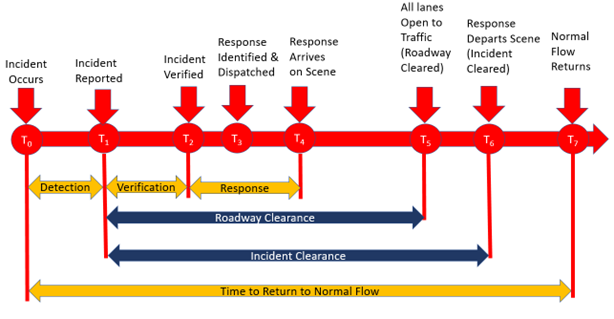
\includegraphics{images/TIM timeline.png}

}

\caption{\label{fig-TIM_Timeline}TIM timeline (adapted from
\citet{conkliin_data_2013}).}

\end{figure}%

The CAD data were adequate to determine the performance measures of RT
and ICT for most incidents but not for RCT, which was obtained from the
UDOT TransSuite database. The TransSuite database includes the
timestamps of lane closures, which were used for the T\textsubscript{5}
timestamp for each incident which TransSuite had the data available. An
Excel Visual Basic for Applications (VBA) script was used to pair
incidents from the CAD dataset and TransSuite dataset within a similar
timeframe as potential matches for the same incident, and potential
matches were evaluated and verified by the research team based on the
locations and details included in both databases for the given incident.
The lane closure data for confirmed matches were then integrated into
the CAD data using a VBA script.

The total number of incidents contained in the 2018 and 2022 datasets
were 1,097 and 1,526, respectively, which were both taken for the months
of March through August. Of these total incidents, the majority were PDO
crashes. PI crashes made up a minor portion and FII crashes made up less
than one percent for both years. Nearly all incidents had an ICT value
and the majority had an RT value, as shown in Table~\ref{tbl-datatype}.
However, only 28 percent of incidents in 2018 and 21 percent of
incidents in 2022 had an available RCT value due to TranSuite only
overlapping with the CAD database for that portion of incidents. This
reduced the total number of incidents with all necessary timestamps and
performance measures (RT, RCT, and ICT) to 283 and 307 incidents for
2018 and 2022, respectively, leaving only 26 percent and 20 percent of
the original number of incidents, respectively.

\begin{longtable}[]{@{}
  >{\centering\arraybackslash}p{(\columnwidth - 8\tabcolsep) * \real{0.2000}}
  >{\centering\arraybackslash}p{(\columnwidth - 8\tabcolsep) * \real{0.2000}}
  >{\centering\arraybackslash}p{(\columnwidth - 8\tabcolsep) * \real{0.2000}}
  >{\centering\arraybackslash}p{(\columnwidth - 8\tabcolsep) * \real{0.2000}}
  >{\centering\arraybackslash}p{(\columnwidth - 8\tabcolsep) * \real{0.2000}}@{}}
\caption{Data Type}\label{tbl-datatype}\tabularnewline
\toprule\noalign{}
\begin{minipage}[b]{\linewidth}\centering
Data Type
\end{minipage} & \begin{minipage}[b]{\linewidth}\centering
2018 Crashes
\end{minipage} & \begin{minipage}[b]{\linewidth}\centering
2018 Percentage
\end{minipage} & \begin{minipage}[b]{\linewidth}\centering
2022 Crashes
\end{minipage} & \begin{minipage}[b]{\linewidth}\centering
2022 Percentage
\end{minipage} \\
\midrule\noalign{}
\endfirsthead
\toprule\noalign{}
\begin{minipage}[b]{\linewidth}\centering
Data Type
\end{minipage} & \begin{minipage}[b]{\linewidth}\centering
2018 Crashes
\end{minipage} & \begin{minipage}[b]{\linewidth}\centering
2018 Percentage
\end{minipage} & \begin{minipage}[b]{\linewidth}\centering
2022 Crashes
\end{minipage} & \begin{minipage}[b]{\linewidth}\centering
2022 Percentage
\end{minipage} \\
\midrule\noalign{}
\endhead
\bottomrule\noalign{}
\endlastfoot
Incidents & 1,097 & 100\% & 1,526 & 100\% \\
ICT & 1,089 & 99\% & 1,520 & \textgreater99\% \\
RT & 944 & 86\% & 1,272 & 83\% \\
RCT & 305 & 28\% & 319 & 21\% \\
ICT, RT, and RCT & 283 & 26\% & 307 & 20\% \\
Incidents Analyzed for User Impacts & 172 & 16\% & 236 & 15\% \\
\end{longtable}

Summary statistics for the performance measures, user impacts, and other
pertinent IMT data of years 2018 and 2022 are compared in
Table~\ref{tbl-SummaryStats}. All performance measures had large
standard deviations from the mean due to the wide range of values
contained for each parameter in the dataset. For IMT performance
measures, the mean of RT decreased from 16.5 minutes in 2018 to 13.8
minutes in 2022, for a difference of 2.7 minutes with a standard error
of 1.1 minute. However, IMT RCT and ICT increased by 8.9 minutes and 3.6
minutes, respectively, from 2018 to 2022, showing that IMTs did not
necessarily clear all lanes of the roadway or leave the crash site any
faster in 2022 than in 2018.

\begin{table}

\caption{\label{tbl-SummaryStats}}

\centering{

\captionsetup{labelsep=none}

\centering
\begin{tabular}[t]{llrrrr}
\toprule
\multicolumn{2}{c}{ } & \multicolumn{2}{c}{2018} & \multicolumn{2}{c}{2022} \\
\cmidrule(l{3pt}r{3pt}){3-4} \cmidrule(l{3pt}r{3pt}){5-6}
  &    & Mean & Std. Dev. & Mean & Std. Dev.\\
\midrule
RT &  & 16.5 & 11.7 & 13.8 & 9.5\\
RCT &  & 41.3 & 32.2 & 50.1 & 39.7\\
ICT &  & 64.0 & 34.8 & 67.6 & 41.3\\
AV &  & 7826.5 & 4939.6 & 6505.8 & 4873.1\\
ETT &  & 845.3 & 1229.5 & 476.5 & 823.6\\
EUC &  & 21725.5 & 32459.5 & 12537.4 & 22698.2\\
T7-T0 &  & 77.0 & 46.3 & 72.5 & 48.9\\
\midrule\\
 &  & N & Pct. & N & Pct.\\
Crash Type & Fatal & 2 & 1.2 & 4 & 1.7\\
 & PD Crash & 89 & 53.0 & 90 & 38.6\\
 & PI Crash & 77 & 45.8 & 139 & 59.7\\
\bottomrule
\end{tabular}

}

\end{table}%

For user impacts of crashes responded to by IMTs, AV decreased from an
average of 7826.5 vehicles affected per crash in 2018 to 6505.8 in 2022,
for a difference of -1320.7 between 2022 and 2018 and a percent
difference of 16.9 percent between 2018 and 2022. While ETT and EUC both
had standard deviations larger than the means due to the wide range of
values included for both parameters, ETT decreased from 845.3 hours of
delay per crash in 2018 to 476.5 in 2022; this is a difference of -368.8
between 2022 and 2018 and a percent difference of 43.6 between 2018 and
2022. EUC decreased from 21,725.50 dollars per crash in 2018 to
12,537.40 in 2022; this is a difference of -9,188.20 between 2022 and
2018 and a percent difference of 42.3 between 2018 and 2022. The
T\textsubscript{7}-T\textsubscript{0} parameter, representing the total
time for which the speed of traffic is significantly reduced, decreased
by about 4.5 minutes between 2018 and 2022.

These initial results for the expansion of the IMT program show that
while IMT RCT and ICT showed no overall improvements that IMT RT
decreased minorly and user impacts decreased significantly. AV decreased
by 16.9 percent, and ETT and EUC both decreased by approximately 43
percent between 2018 and 2022. A brief description of how user impacts
were obtained is presented hereafter.

\subsection{User Impacts}\label{user-impacts}

User impacts were quantified for all incidents that had a decipherable
queue and no secondary incidents whose queue affected that of the
primary incident. Incidents were evaluated for user impacts by obtaining
UDOT traffic data for roadway at the time and location of the incident
as well as for the same location but on normal days when an incident did
not occur to establish baseline conditions. The stretch of the roadway
where traffic was affected by a crash was then segmented into subroutes
between ramps to evaluate the time when the average speed of traffic
first decreased significantly below normal (T\textsubscript{0}) and when
it returned to within normal (T\textsubscript{7}) to a granularity of 5
minutes. The AV of each subroute was taken as the sum of the volume of
vehicles between T\textsubscript{0} and T\textsubscript{7} for the
incident day, and the AV of the incident was taken to be the maximum AV
of all subroutes affected by the crash. The effects of diversion were
not included in this analysis.

The ETT of an incident was found by calculating the ETT for each
5-minute increment between T\textsubscript{0} and T\textsubscript{7} for
the incident and average of normal days. The hours of ETT for each
5-minute increment were found by multiplying the average travel time of
the subroute by the volume of vehicles at that loop detector. The ETT of
an incident was then calculated by taking the difference between the sum
of the ETT for each 5-minute increment between T\textsubscript{0} and
T\textsubscript{7} for the incident and average of normal days.

EUC is the sum of the cost of ETT for passenger vehicles and trucks.
Costs due to the ETT of passengers and trucks are the only factors
considered in this analysis. The formula used for EUC is shown below
where the percent trucks (T) was the portion of vehicles over 30 ft in
length obtained from UDOT Traffic Data; the average vehicle occupancy
(AVO) was taken as 1.14 for the I-15 based on
\citet{schultz_ut1503_2015}; the individual hourly cost (IHC) and truck
hourly cost (THC) were taken as \$17.81 and \$53.69 based on
\citet{ellis_value_2017}. While the IHC and THC are somewhat outdated
for the 2022 data, these values were still used to be consistent with
2018 EUC values to make a valid comparison free of the effects of
inflation.

\[EUC = ETT \times ((1-T) \times AVO \times IHC + T \times THC) \]

\subsection{Models}\label{models}

This study hypothesizes that the expanded IMT program was the primary
cause for the reduction in user impacts as well as IMT RT. The dependent
variables considered in this analysis were the natural log of all user
impacts (\emph{Ln AV}, \emph{Ln ETT}, and \emph{Ln EUC}), the natural
log of RCT (\emph{Ln RCT}) and IMT ICT (\emph{Ln ICT}), and IMT
\emph{RT}. Due to the data distribution for all user impacts and most
performance measures being right-skewed, or skewed towards large
outliers, it was determined that a natural log (Ln) transformation would
be taken to better fit the user impacts and performance measures data
with the exception of \emph{RT}, for which a natural log transformation
did not help better describe the data for this variable. The independent
variables considered for performance measures were incident
characteristics described below. The independent variables considered
for user impacts were \emph{Ln T\textsubscript{7}-T\textsubscript{0}},
performance measures, and incident characteristics.

The first incident characteristics considered in the models for this
analysis was the \emph{Year}. The years for which crash data were
analyzed were 2018 (reference case) and 2022, explaining the difference
in user impacts and IMT performance based on IMT program size before and
after the expansion. This was treated as a categorical variable. The
\emph{Crash Type} variable was included due to it accounting for some
significant differences in crash data; the crash types included as
mentioned previously are PDO, PI (reference), and FII. It should be
noted that FII crashes had a very small sample size, thus skewing many
of the results due to the irregular nature of these crashes and the
complications introduced by them to incident response protocol.

The \emph{Time Range} variable was included; crashes analyzed for user
impacts were divided into the following time ranges:

\begin{itemize}
\item
  Morning Off Peak (Morning): 11:45 PM to 5:30 AM
\item
  AM Peak: 5:30 AM to 9:00 AM
\item
  Afternoon Off Peak (Afternoon) (Reference case): 9:00 AM to 3:45 PM
\item
  PM Peak: 3:45 PM to 6:15 PM
\item
  Night Off Peak (Night): 6:15 PM to 11:45 PM
\end{itemize}

The \emph{Number of (N.) IMTs} that responded to a crash was included.
Note that this is a reactionary variable; IMT protocol was to dispatch
one team for crash response for most incidents or two teams for more
severe incidents. Additional teams were sent based on crash severity and
IMT availability rather than an anticipated number being sent initially.
A variable similar in nature to this that was also included in the
analysis was the \emph{Number of (N.) UHPs Teams} that responded to a
crash. These parameters were both found to be correlated with IMT
performance measures but not as well with user impacts.

The \emph{Number of (N.) Lanes Closed} at any point during incident
response was well correlated with ETT. A similar variable that was
quantified to further investigate the effect of IMTs clearing a lane at
any given time was the time weighted number of lanes closed
(\emph{TWNLC}). This is the time weighted average of the number of lanes
closed during incident response, which was initially hypothesized to
more precisely determine the user impacts of a crash. This was
calculated using the following formula where t\textsubscript{i} is the
number of minutes that each given lane i was closed (0 minutes for lanes
that were not closed), N is the number of lanes at the bottleneck of the
crash, and t\textsuperscript{*} is the total time for which any lane of
the roadway was closed during an incident. One limitation of this
parameter is that not all incidents analyzed for user impacts had all
lane closures clearly defined without errors in the data to clearly
determine \emph{TWNLC}, therefore only 379 incidents of the 401 total
number of incidents analyzed for user impacts (95 percent) could be
analyzed for this parameter.

\[ TWNLC = \frac{\sum_{i=1}^{N}t_i}{N \times t^*}
\]

The \emph{Total Number of (Total) Lanes} at the bottleneck of a crash
was included for user impacts analysis as it was correlated with AV. The
dominant independent variable for user impacts was \emph{Ln
T\textsubscript{7}-T\textsubscript{0}}, or the natural log of the
difference between the time when the average speed of traffic during an
incident returned to within approximately 20 mph of the average speed at
normal conditions (T\textsubscript{7}) and the time when the incident
occurred (T\textsubscript{0}). This is effectively the incident duration
for which roadway users are impacted. A logarithmic transformation was
applied due to the right-skew of the data and to achieve best fit in
linear regression.

The model groups analyzed to evaluate the UDOT IMT program expansion are
as follows, \[ 
{PM}_i = {Year}_i + {TR}_i + {CT}_i + X_i\beta
\] and \[ 
{UI}_i = {Year}_i + {TR}_i + {CT}_i + {Ln(T_7 -T_0)}_i\beta + {PM}_i\beta + X_i\beta
\]

where the variable index \(i\) denotes being for a single incident, PM
is performance measure, TR is time range, CT is crash type, and \(X\) is
a vector of the other incident characteristics variables not listed
above, and \(\beta\) are estimated coefficients. While various models
were evaluated for each performance measure and user impact, only those
with most meaningful results are presented hereafter.

\bookmarksetup{startatroot}

\section{Results}\label{results}

The purpose of this section is to present the results of the regression
analysis of the UDOT IMT program expansion. The IMT performance measures
of RT, \emph{Ln RCT}, and \emph{Ln ICT} were analyzed with incident
characteristics as independent variables. RT was only the performance
measure shown to have improved due to the expansion of the IMT program.
The user impacts of Ln AV, Ln ETT, and Ln EUC were also analyzed with
both performance measures and incident characteristics as independent
variables. Overall, user impacts have many more variables that explain
them with significantly better fit than do performance measures with the
prime variable being \emph{Ln T\textsubscript{7}-T\textsubscript{0}},
representing the natural log transformed total time which an incident
significantly decreases the average speed of traffic.

\subsection{Performance Measures}\label{performance-measures}

The IMT performance measures of \emph{RT}, \emph{Ln RCT}, and \emph{Ln
ICT} were analyzed against several incident characteristics. Overall,
the program expansion results in minor improvements in RT but not for
RCT and ICT. However, the analysis of performance measures provides
models with a similar R\textsuperscript{2} value to those of robust
previous studies such as \citet{mumtarin_traffic_2023} using continuous
variables such as \emph{N. of IMTs} and \emph{TWNLC}, which provide a
significantly better overall fit compared to the non-continuous
variables of crash type and time range, as shown in the models of this
subsection.

\emph{RT} is primarily described by the \emph{N. of IMTs} and
\emph{TWNLC}, which variables are included in the statistical models in
Table~\ref{tbl-rtmodels}. The year 2018 variable indicates that IMTs
took approximately 2.7 minutes longer to respond to crashes in 2018
before the expansion than in 2022 when there were more units. The
\emph{N. of IMTs} variable indicates that \emph{RT} decreased by
approximately 1.5 minutes for each added IMT that responded to an
incident, showing that crashes where more IMTs were required were
treated more urgently after detection than those where fewer IMTs
responded.

The \emph{TWNLC} coefficient of 1.931 minutes indicates that IMTs took
almost 2 minutes longer to respond for each 1.0 incremental increase in
the average number of lanes closed throughout the crash. This suggests
that IMTs could not reach the crash site as quickly due to congestion
when more lanes were closed. Models where \emph{Ln RCT}, \emph{Ln ICT},
and user impacts were included also showed that each of the mentioned
variables had a positive correlation with \emph{RT}, indicating that it
took IMTs longer to respond to incidents that took longer to clear and
greater user impacts.

The time range variable was only statistically significant for the
Morning Off Peak range, which time range had a least squares means
average of between 39 and 42 minutes longer \emph{RT} values than other
time ranges; this accounts for outlier incidents where IMTs took
significantly longer to respond to crashes in the early morning than in
the afternoon off peak and other time periods due to fewer IMTs and UHP
teams working during this period. The lanes closed and crash type
variables were also analyzed but did not help to improve the fit of the
model or help further explain differing values of \emph{RT}. The
\emph{Year} variable was interacted with the variables included in the
models in Table~\ref{tbl-rtmodels} and other variables; however, no
statistically significant interactions were found, showing that no other
variables quantified in this study had a statistically significant
effect on the difference in \emph{RT} due to the program expansion.

\begin{table}

\caption{\label{tbl-rtmodels}Estimated Models of IMT RT}

\centering{

\centering
\begin{tabular}[t]{lcc}
\toprule
  & Base & TWNLC\\
\midrule
(Intercept) & 15.657*** & 13.716***\\
 & (1.423) & (1.662)\\
Year 2018 (ref. 2022) & 2.737** & 2.673*\\
 & (1.009) & (1.040)\\
Morning (ref. Afternoon) & 42.974*** & 39.110***\\
 & (4.838) & (5.033)\\
AM Peak (ref. Afternoon) & -1.454 & -1.645\\
 & (1.299) & (1.336)\\
PM Peak (ref. Afternoon) & 0.643 & 0.117\\
 & (1.179) & (1.219)\\
Night (ref. Afternoon) & 0.362 & -0.468\\
 & (2.071) & (2.206)\\
N. IMTs & -1.476* & -1.978**\\
 & (0.698) & (0.751)\\
TWNLC &  & 1.931**\\
 &  & (0.692)\\
\midrule
Num.Obs. & 384 & 362\\
R2 & 0.201 & 0.220\\
R2 Adj. & 0.188 & 0.205\\
\bottomrule
\multicolumn{3}{l}{\rule{0pt}{1em}+ p $<$ 0.1, * p $<$ 0.05, ** p $<$ 0.01, *** p $<$ 0.001}\\
\multicolumn{3}{l}{\rule{0pt}{1em}Dependent variable: RT}\\
\multicolumn{3}{l}{\rule{0pt}{1em}Standard errors in parentheses}\\
\end{tabular}

}

\end{table}%

Models of \emph{Ln RCT} confirmed the results of the descriptive
statistics in Table~\ref{tbl-SummaryStats} that there was a minor
statistically significant difference between RCT in 2022 and 2018 where
2022 RCT values were greater than in 2018. As mentioned previously, this
was hypothesized to have been affected by the greater percentage of PI
crashes than PDO crashes in 2022 than in 2018 and the protocol during
the COVID-19 pandemic to emphasize safety. The \emph{Crash Type}
variable in \emph{Ln RCT models} was found to be statistically
significant where PDO crashes were found to have RCT values
approximately 32 percent less than those of PI crashes. A \emph{Year
2018*PDO Crash} interaction variable was included in one model but not
found to be statistically significant. Models of \emph{Ln ICT} showed
that there was no statistically significant difference between values in
2018 and 2022. These models show that the program expansion did not
reduce IMT RCT and ICT as it did RT and user impacts. Both \emph{Ln RCT}
and \emph{Ln ICT} were primarily explained by the \emph{N. IMTs} and
\emph{N. UHP Teams} variables; \emph{RT} and \emph{Crash Type} had a
minor impact on \emph{Ln RCT} and \emph{Ln ICT} values and helped to fit
the model to approximately the same adjusted R\textsuperscript{2} value
as for IMT RT. The \emph{Time Range} variable was not statistically
significant for either variable.

\subsection{User Impacts}\label{user-impacts-1}

The user impact variables of \emph{Ln AV}, \emph{Ln ETT}, and \emph{Ln
EUC} are modeled in this subsection to demonstrate the impact of the
UDOT IMT program expansion and identify the variables that best describe
each user impact. The fit of statistical models for user impacts
variables was consistently better than that for performance measures due
to user impacts having more variables of close fit available in the
crash data set that describe phenomenons occurring during crashes.

\emph{Ln AV} is best described by the dominant variable of \emph{Ln
T\textsubscript{7}-T\textsubscript{0}} as well as the \emph{Total Lanes}
variable. The base model of Table~\ref{tbl-avmodels}, which includes
\emph{Ln T\textsubscript{7}-T\textsubscript{0}} as the only continuous
variable along with all categorical variables, explains the majority of
the data with an adjusted R\textsuperscript{2} value of 0.69 that
increases moderately with the addition of other variables and
interaction terms in following models. This indicates that the number of
vehicles affected by a crash is best explained by the time for which the
speed of traffic is reduced significantly below normal during an
incident. The coefficient of \emph{Ln
T\textsubscript{7}-T\textsubscript{0}} in the ``Base'' model of 0.906
indicates that the increase in the number of vehicles affected by a
crash without being affected by other variables is equal to the
multiplicative increase in \emph{Ln
T\textsubscript{7}-T\textsubscript{0}} raised to the 0.906 power. For
example, if T\textsubscript{7}-T\textsubscript{0} increases by 10
percent for a given incident, or a factor of 1.1, then AV will increase
by a factor of 1.1\textsuperscript{0.906}, or approximately 1.09, or if
T\textsubscript{7}-T\textsubscript{0} increases by 50 percent for the
same incident, then AV will increase by a factor of
1.5\textsuperscript{0.906}, or approximately 1.44.

\begin{table}

\caption{\label{tbl-avmodels}Estimated Models of Ln AV}

\centering{

\centering
\begin{tabular}[t]{lcccc}
\toprule
  & Base & Int. 1 & T. Lanes & Int. 2\\
\midrule
(Intercept) & 4.813*** & 4.994*** & 3.924*** & 3.766***\\
 & (0.143) & (0.177) & (0.143) & (0.153)\\
Year 2018 (ref. 2022) & 0.107* & -0.372 & 0.128*** & 0.553***\\
 & (0.043) & (0.280) & (0.036) & (0.161)\\
PDO Crash (ref. PI) & 0.093* & 0.090* & 0.073* & 0.075*\\
 & (0.042) & (0.042) & (0.036) & (0.036)\\
FII Crash (ref. PI) & -0.642*** & -0.615** & -0.636*** & -0.643***\\
 & (0.187) & (0.187) & (0.160) & (0.158)\\
Morning (ref. Afternoon) & -0.765*** & -0.811*** & -0.807*** & -0.782***\\
 & (0.225) & (0.226) & (0.192) & (0.191)\\
AM Peak (ref. Afternoon) & 0.006 & 0.013 & 0.040 & 0.030\\
 & (0.055) & (0.055) & (0.047) & (0.047)\\
PM Peak (ref. Afternoon) & 0.115* & 0.116* & 0.134** & 0.128**\\
 & (0.049) & (0.049) & (0.042) & (0.042)\\
Night (ref. Afternoon) & -0.487*** & -0.507*** & -0.491*** & -0.493***\\
 & (0.089) & (0.090) & (0.076) & (0.076)\\
Ln T7-T0 & 0.906*** & 0.862*** & 0.895*** & 0.897***\\
 & (0.033) & (0.042) & (0.028) & (0.028)\\
Ln T7-T0*2018 &  & 0.116+ &  & \\
 &  & (0.067) &  & \\
Total Lanes &  &  & 0.177*** & 0.207***\\
 &  &  & (0.015) & (0.018)\\
Total Lanes*2018 &  &  &  & -0.082**\\
 &  &  &  & (0.030)\\
\midrule
Num.Obs. & 400 & 400 & 400 & 400\\
R2 & 0.699 & 0.701 & 0.781 & 0.785\\
R2 Adj. & 0.693 & 0.694 & 0.776 & 0.779\\
\bottomrule
\multicolumn{5}{l}{\rule{0pt}{1em}+ p $<$ 0.1, * p $<$ 0.05, ** p $<$ 0.01, *** p $<$ 0.001}\\
\multicolumn{5}{l}{\rule{0pt}{1em}Dependent variable: Ln AV}\\
\multicolumn{5}{l}{\rule{0pt}{1em}Standard errors in parentheses}\\
\end{tabular}

}

\end{table}%

The \emph{Year 2018} variable in the ``Base'' model is moderately
statistically significant with a coefficient of 0.107, which indicates
that the number of vehicles affected by crashes responded to by IMTs in
2018 that is not accounted for by other variables is higher than that of
2022 by a factor of e\textsuperscript{0.107}, or 1.11. This suggests
that the IMT program expansion with an increased number of units
covering Utah roadways decreased the number of vehicles affected by
crashes responded to by IMTs by approximately 11 percent. Another
variable controlled for is the change in Ln
T\textsubscript{7}-T\textsubscript{0} between 2018 and 2022 with the
addition of a \emph{Year 2018*Ln T\textsubscript{7}-T\textsubscript{0}}
added to the ``Interaction 1'' model. This variable being suggestively
statistically significant indicates that there is somewhat of a
difference in the log-linear slope of Ln AV vs \emph{Ln
T\textsubscript{7}-T\textsubscript{0}} in 2018 from the reference case
of 2022, as shown in \textbf{?@fig-LnAVvsLnT7T0\_year}. A positive
coefficient of 0.116 indicates that an increase in
T\textsubscript{7}-T\textsubscript{0} will have a slightly greater
effect in 2018 than in 2022, where a 10 percent increase in the
T\textsubscript{7}-T\textsubscript{0} would cause the AV of a 2018 crash
to be 1.1\textsuperscript{0.116}, or 1.01, times higher than that of
2022. Note that the \emph{Year 2018} variable for this model and each
model with a \emph{Year 2018} interaction variable are both
statistically non-significant and have a negative value in this model
and other models with a \emph{Year 2018} interaction due to the
log-linear slope being slightly greater in 2018 causing a downward shift
to the \emph{Year 2018} plus intercept for 2018 crashes.

\includegraphics{04_results_files/figure-pdf/unnamed-chunk-2-1.pdf}

The \emph{Total Lanes} coefficient in the ``Total Lanes'' model
indicates that each added lane at the bottleneck of a crash results in
an increase in AV by a factor of e\textsuperscript{0.177}, or 1.19, due
to roads with more lanes having significantly higher volumes of vehicles
that may be impacted by a crash. The T\emph{otal Lanes*Year 2018}
interaction variable indicates a lower log-linear slope for 2018 crashes
for \emph{Ln AV} vs \emph{Total Lanes}, showing that 2018 crashes were
less sensitive to the number of lanes at the bottleneck of a crash.
However, the effect is minor with each added lane at the bottleneck of a
crash being only reducing the AV of 2018 crashes by a multiplicative
difference of e\textsuperscript{-0.082}, or 0.92, from that of 2022
crashes. No performance measures were statistically significant when
modeled with \emph{Ln AV} when the \emph{Ln
T\textsubscript{7}-T\textsubscript{0}} variable was present due to most
performance measures being colinear with \emph{Ln
T\textsubscript{7}-T\textsubscript{0}} but not adding much further
explanation to \emph{Ln AV}.

Models of \emph{Ln ETT} are shown in Table~\ref{tbl-ettmodels1}. Each
model without a \emph{Year 2018} interaction variable (which would
change the difference from the intercept) has a coefficient value of
between 0.4 and 0.5, indicating that crashes in 2018 experienced greater
ETT by a factor of between e\textsuperscript{0.4} and
e\textsuperscript{0.5}, or 1.49 and 1.65, due to the increased number of
IMTs in the program. This shows that while the number of vehicles
affected by a crash in 2022 is reduced minorly by 11 percent from 2018
that the delay experienced by all users collectively decreases by
approximately 50 percent for the reference case of PI crashes. The PDO
\emph{Crash Type} variable is not statistically significant in any
\emph{Ln ETT} model and has a low coefficient, indicating that the
reduction in delay for PI crashes is also relatively the same for PDO
crashes.

As for the \emph{Ln AV} models, \emph{Ln
T\textsubscript{7}-T\textsubscript{0}} explains the majority of the ETT
experienced by roadway users, while other variables further explain
variations in \emph{Ln ETT} for different crash scenarios. The \emph{Ln
T\textsubscript{7}-T\textsubscript{0}} coefficient in the ``Base'' model
of 1.911 indicates that a 10 percent increase in
T\textsubscript{7}-T\textsubscript{0}, or the time for which the average
speed of traffic is reduced significantly below normal, results in an
increase in ETT by a factor of 1.1\textsuperscript{1.911}, or 1.20,
showing that a 10 percent increase results in a 20 percent increase in
the delay experienced by all users. The following models with lower
\emph{Ln T\textsubscript{7}-T\textsubscript{0}} coefficients due to
other variables helping to explain ETT indicate that for the same 10
percent increase in T\textsubscript{7}-T\textsubscript{0} that it would
result in a multiplicative increase in ETT ranging from
1.1\textsuperscript{1.21} to 1.1\textsuperscript{1.77}, or from 1.12 to
1.18, depending on the variables including interaction terms included in
the model. An \emph{Ln T\textsubscript{7}-T\textsubscript{0}*Year 2018}
interaction variable was included in one model but was not statistically
significant, showing that the difference between the length of
T\textsubscript{7}-T\textsubscript{0} in 2018 and 2022 did not have a
significant impact on the delay experienced by roadway users.

\begin{table}

\caption{\label{tbl-ettmodels1}Estimated Models of Ln ETT}

\centering{

\centering
\begin{tabular}[t]{lccccc}
\toprule
  & Base & RCT & TWNLC & Lanes & Int.\\
\midrule
(Intercept) & -2.716*** & -2.913*** & -3.101*** & -2.935*** & -3.100***\\
 & (0.388) & (0.393) & (0.393) & (0.370) & (0.381)\\
Year 2018 (ref. 2022) & 0.454*** & 0.498*** & 0.538*** & 0.505*** & 0.842***\\
 & (0.115) & (0.116) & (0.114) & (0.109) & (0.221)\\
PDO Crash (ref. PI) & -0.067 & 0.002 & 0.004 & 0.000 & 0.002\\
 & (0.115) & (0.117) & (0.115) & (0.110) & (0.110)\\
FII Crash (ref. PI) & -1.398** & -1.567** & -2.285*** & -1.986*** & -1.997***\\
 & (0.506) & (0.507) & (0.498) & (0.481) & (0.479)\\
Morning (ref. Afternoon) & -1.234* & -1.249* & -1.724** & -1.866** & -1.785**\\
 & (0.608) & (0.604) & (0.581) & (0.575) & (0.575)\\
AM Peak (ref. Afternoon) & 0.095 & 0.089 & 0.101 & 0.027 & 0.037\\
 & (0.149) & (0.148) & (0.145) & (0.140) & (0.139)\\
PM Peak (ref. Afternoon) & 0.453*** & 0.483*** & 0.466*** & 0.459*** & 0.467***\\
 & (0.132) & (0.132) & (0.130) & (0.124) & (0.124)\\
Night (ref. Afternoon) & -1.472*** & -1.492*** & -1.789*** & -1.719*** & -1.729***\\
 & (0.242) & (0.240) & (0.242) & (0.228) & (0.228)\\
Ln T7-T0 & 1.911*** & 1.773*** & 1.645*** & 1.625*** & 1.626***\\
 & (0.089) & (0.105) & (0.104) & (0.101) & (0.100)\\
Ln RCT &  & 0.203* & 0.192* & 0.183* & 0.185*\\
 &  & (0.082) & (0.082) & (0.077) & (0.077)\\
TWNLC &  &  & 0.484*** &  & \\
 &  &  & (0.077) &  & \\
N. Lanes Closed &  &  &  & 0.371*** & 0.444***\\
 &  &  &  & (0.052) & (0.066)\\
N. Lanes Closed*2018 &  &  &  &  & -0.169+\\
 &  &  &  &  & (0.096)\\
\midrule
Num.Obs. & 400 & 400 & 378 & 400 & 400\\
R2 & 0.616 & 0.622 & 0.653 & 0.666 & 0.669\\
R2 Adj. & 0.608 & 0.613 & 0.643 & 0.657 & 0.659\\
\bottomrule
\multicolumn{6}{l}{\rule{0pt}{1em}+ p $<$ 0.1, * p $<$ 0.05, ** p $<$ 0.01, *** p $<$ 0.001}\\
\multicolumn{6}{l}{\rule{0pt}{1em}Dependent variable: Ln ETT}\\
\multicolumn{6}{l}{\rule{0pt}{1em}Standard errors in parentheses}\\
\end{tabular}

}

\end{table}%

The \emph{Ln RCT} variable being added in the ``Ln RCT'' model does not
have a large impact on ETT with a 10 percent increase in RCT resulting
in a multiplicative increase in ETT of only 1.1\textsuperscript{0.203},
or 1.02. \emph{RT} and \emph{Ln ICT} did not have a statistically
signficant effect on any Ln ETT models. The ``TWNLC'' model indicates
that each added increment of 1.0 to \emph{TWNLC} causes ETT to increase
by a multiplicative difference of e\textsuperscript{0.484}, or 1.62,
showing that the impact of the total time for which a lane is closed has
significant impacts on ETT. The ``N. Lanes Closed'' model represents a
similar phenomenon but where the lane variable is the number of lanes
closed at any given time during an incident rather than the time
weighted average (\emph{TWNLC}). The \emph{N. of Lanes Closed}
coefficient of 0.376 indicates that for each lane closed at any point
during incident response that \emph{Ln ETT} increases by a factor of
e\textsuperscript{0.376}, or 1.46, showing that an additional lane
closed for any amount of time during an incident results in
significantly higher delay for roadway users, though not as much as one
closed for the duration of the crash response versus at all.

The \emph{N. Lanes Closed*Year 2018} interaction variable coefficient of
-0.169 indicates that the effect of an added lane in 2018 results in
less added ETT than in 2022 by a factor of e\textsuperscript{-0.169}, or
0.84. This shows that the log-linear slope of \emph{Ln ETT} vs \emph{N.
of Lanes Closed} is lower in 2018 and that crashes in this year were
slightly less sensitive to the effects of an additional lane closed than
2022.

Because EUC is defined as being a function of ETT that is adjusted only
for AVO and the percentage of trucks on the roadway, \emph{Ln EUC} and
\emph{Ln ETT} are highly correlated with and proportional to one
another. Therefore, the coefficients in the \emph{Ln EUC} models were
virtually the same as those in Table~\ref{tbl-ettmodels1} with minor
insignificant differences. Therefore, all trends discussed previously on
\emph{Ln ETT} models are applicable to \emph{Ln EUC} models. The program
expansion thus caused a decrease of 50 percent in the time cost that
users experienced between 2018 and 2022 crashes, demonstrating the
significant benefits that an expanded IMT program has for roadway users
in Utah and in general.

\bookmarksetup{startatroot}

\section{Conclusions}\label{conclusions}

The purpose of this research was to evaluate the benefits of UDOT's
expanded IMT program by evaluating and comparing IMT performance
measures for all crashes in 2018 and 2022 that were responded to by IMTs
as well as the user impacts for those corresponding crashes. Regression
models provided better understanding of the incident characteristics and
crash variables that have the greatest impact on performance measures
and user impacts.

The \emph{Year 2018} variable represents the difference in crash data of
the IMT program between years 2018 and 2022 between which time the
program expanded from 13 units to 25 units. The results of the analysis
of this variable show that there was a statistically significant
difference between IMT RT in 2018 and 2022 of approximately 2.7 minutes
between the two years. This demonstrates that the expansion allows IMTs
to respond faster to crashes presumably due to there being more of them
covering the study area. The variables with the greatest effect on
\emph{RT} were the number of IMTs (\emph{N. IMTs}) that responded to an
incident and \emph{TWNLC}, where each additional IMT that responded was
correlated with approximately 2.0 minutes less RT, and each added lane
that was closed for the duration of the incident was correlated with an
added 1.9 minutes of RT; this also includes the effect of the number of
IMTs within the same model.

RCT and ICT did not have any statistically significant improvements due
to the program expansion, likely due to the IMTs emphasizing safety as
part of post-COVID-19 pandemic protocols and an increase in the
proportion of PI crashes to PDO crashes in 2022. The variables that were
shown to best explain these performance measures were the \emph{N. IMTs}
and \emph{N. UHP Teams} that responded to a an incident as well as
\emph{RT}. While each of the variables mentioned previously were
continuous variables, the \emph{Time Range} variable (categorical)
provided added meaning to the model by eliminating outliers in the
morning off peak period.

Each user impact had a statistically significant and practically
significant \emph{Year 2018} variable coefficient that showed that AV
decreased by approximately 11 percent between 2018 and 2022 and that
both ETT and EUC decreased by approximately 50 percent due to the added
number of IMTs in the program. This shows that more IMTs responding to
more crashes made a moderate reduction to the number of vehicles who
experienced delay for a given crash but made a major reduction in the
total delay and time cost experienced per by all roadway users who
experienced delay in a given crash.

One of the limitations of the \emph{Year 2018} variable is that this
accounts for all differences between 2018 and 2022 variables not
accounted for by other variables, and while it is assumed to primarily
account for the difference in IMT program size and the number of units
on the road, it may not account for the effect of post-pandemic traffic
conditions even though traffic flow rates have largely returned to
normal..

The key independent variables that explain user impacts of incidents
responded to by IMTs are shown in the table below. The impact of each
variable includes the effects of T\textsubscript{7}-T\textsubscript{0}
(which had a natural log transformation applied to the variable due to
the non-linear trends observed in the data). The independent variables
which had a natural log transformation taken for them are interpreted
relatively in percent changes rather than in units of time due to their
effect on user impacts being non-linear. For the purpose of summarizing
the impacts of each variable, a 10 percent increase of the independent
variable was used to make a standard comparison. See the individual
model coefficients and the discussion on back-transforming the variables
with natural log transformations applied for predicting incident
specific effects in Chapter 3.

For T\textsubscript{7}-T\textsubscript{0}, a 10 percent increase
resulted in a 9 percent increase in AV; the \emph{Ln
T\textsubscript{7}-T\textsubscript{0}*Year 2018} variable indicated a
difference of only 1 percent the effect of
T\textsubscript{7}-T\textsubscript{0} on AV in 2018 and 2022.
T\textsubscript{7}-T\textsubscript{0} had a greater impact on ETT and
EUC of a 20 percent increase per 10 percent increase in
T\textsubscript{7}-T\textsubscript{0} when analyzed individually and a
17 percent increase when the effects of the variables \emph{Ln RCT} and
either \emph{TWNLC} or \emph{N. Lanes Closed} were included. This
demonstrates that the time for which speed of traffic is reduced
significantly below normal is the primary independent variable
influencing delay. The \emph{Ln
T\textsubscript{7}-T\textsubscript{0}*Year 2018} variable was not
statistically significant for ETT and EUC, showing that the effect of
the IMT program expansion on The
\emph{T\textsubscript{7}-T\textsubscript{0}} did not have a significant
impact on ETT and EUC.

RCT did not have a statistically significant impact on AV when analyzed
in the same model as T\textsubscript{7}-T\textsubscript{0}; while it was
a statistically significant variable for ETT and EUC, it only increased
these by 2 percent for each 10 percent increase in RCT. The number of
lanes closed and TWNLC were not found to have a statistically
significant effect on AV. However, the impact of 1 additional lane
closed at any point during an incident increased ETT and EUC by 45
percent, and the impact of 1 additional lane closed for the duration of
an incident increased ETT and EUC by 62 percent. The variable other than
T\textsubscript{7}-T\textsubscript{0} that was found to have the
greatest impact on AV was the total number of lanes at the bottleneck of
a crash, which caused a 19 percent increase in AV and 21 percent
increase in ETT and EUC for each added lane. This demonstrates that the
number of lanes closed at any point during an incident and the time for
which they are closed have a large impact on the delay experienced by
roadway users while the total number of lanes is better correlated with
the number of roadway users affected by a crash.

\begin{longtable}[]{@{}
  >{\raggedright\arraybackslash}p{(\columnwidth - 4\tabcolsep) * \real{0.2976}}
  >{\raggedright\arraybackslash}p{(\columnwidth - 4\tabcolsep) * \real{0.2798}}
  >{\raggedright\arraybackslash}p{(\columnwidth - 4\tabcolsep) * \real{0.4226}}@{}}
\caption{Impact of Independent Variables on User Impacts with the
effects of T\textsubscript{7}-T\textsubscript{0}
included}\tabularnewline
\toprule\noalign{}
\begin{minipage}[b]{\linewidth}\raggedright
Independent Variable
\end{minipage} & \begin{minipage}[b]{\linewidth}\raggedright
AV
\end{minipage} & \begin{minipage}[b]{\linewidth}\raggedright
ETT and EUC
\end{minipage} \\
\midrule\noalign{}
\endfirsthead
\toprule\noalign{}
\begin{minipage}[b]{\linewidth}\raggedright
Independent Variable
\end{minipage} & \begin{minipage}[b]{\linewidth}\raggedright
AV
\end{minipage} & \begin{minipage}[b]{\linewidth}\raggedright
ETT and EUC
\end{minipage} \\
\midrule\noalign{}
\endhead
\bottomrule\noalign{}
\endlastfoot
T\textsubscript{7}-T\textsubscript{0} & 9\% increase per 10\% increase
in T\textsubscript{7}-T\textsubscript{0} & 17-20\% increase per 10\%
increase in T\textsubscript{7}-T\textsubscript{0} (see regression
models) \\
RCT & NA & 2\% increase per 10\% increase in RCT \\
N. of Lanes Closed & NA & 45\% increase per added lane closed at any
point during the crash \\
Time Weighted Number of Lanes Closed (TWNLC) & NA & 65\% increase per
added lane closed for the duration of the crash \\
Total Number of Lanes at the Bottleneck of Crash & 19\% increase per
added lane at the bottleneck & 21\% increase per added lane at the
bottleneck \\
\end{longtable}

This study is the first of its kind to analyze both IMT performance
measures and user impacts for detailed crash data to evaluate the
expansion of an existing IMT program. The findings on the expansion of
UDOT's IMT program provides a valuable reference point for other
transportation agencies potentially considering expanding their own
program due to the significant benefits of significantly reduced user
impacts associated with additional IMTs responding to more crashes
within a given coverage area.

This study also highlights the crash data variables that have the
greatest impacts on IMT performance measures and user impacts to help
provide a better understanding to the field of TIM researchers and
professionals. While other studies have performed detailed analysis on
performance measures given incident characteristics, few studies have
incorporated RT to model RCT and ICT. Fewer studies have been conducted
on delay and user impacts associated with crashes responded to by IMTs
using detailed incident data instead of simulation models, and the
findings from this study provide well-fitted, simplistic models
reflecting the impacts of incident characteristics and IMT performance
measures on user impacts.

\bookmarksetup{startatroot}

\section*{References}\label{references}
\addcontentsline{toc}{section}{References}

\markboth{References}{References}

\renewcommand{\bibsection}{}
\bibliography{references.bib,IMTRegression.bib}




\end{document}
